\def\layersep{2cm}
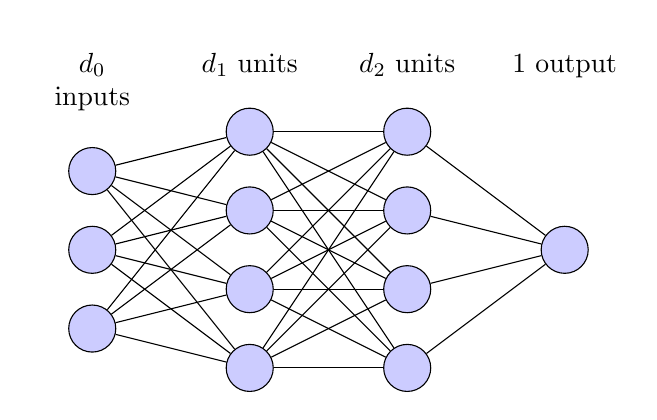
\begin{tikzpicture}[-,draw=black, node distance=\layersep]
    \tikzstyle{neuron}=[circle,draw=black,minimum size=17pt,inner sep=0pt,fill={rgb,255:red,204;green,204;blue,255}]
    \tikzstyle{annot} = [text width=4em, text centered, text height=3ex, text depth=3ex]

    \foreach \name / \y in {1,...,3}
        \node[neuron] (I-\name) at (0,-\y) {};

    \foreach \name / \y in {1,...,4}
        \path[yshift=0.5cm]
            node[neuron] (H-\name) at (\layersep,-\y cm) {};
            
    \foreach \name / \y in {1,...,4}
        \path[yshift=0.5cm]
            node[neuron] (H1-\name) at (\layersep*2,-\y cm) {};

    \node[neuron] (O) at (\layersep*3,-2 cm) {};

    \foreach \source in {1,...,3}
        \foreach \dest in {1,...,4}
            \path (I-\source) edge (H-\dest);
            
    \foreach \source in {1,...,4}
        \foreach \dest in {1,...,4}
            \path (H-\source) edge (H1-\dest);

    \foreach \source in {1,...,4}
        \path (H1-\source) edge (O);

    \node[annot,above of=H-1, node distance=0.75cm] (hl) {$d_1$ units};
    \node[annot,left of=hl] {$d_0$ inputs};
    \node[annot,right of=hl] (h2) {$d_2$ units};
    \node[annot,right of=h2] {$1$ output};
\end{tikzpicture}